% The valid clause gadgets with four auxiliary vertices, one per class
% (see README.md in this folder). Build: pdflatex four-auxiliary-gadgets.tex
\documentclass[varwidth=11.6cm,border=8pt]{standalone}
\usepackage{tikz}
\newcommand{\GT}{G_{\mathrm{T}}}
\newcommand{\GF}{G_{\mathrm{F}}}
\newcommand{\GB}{G_{\mathrm{B}}}
\begin{document}
\centering
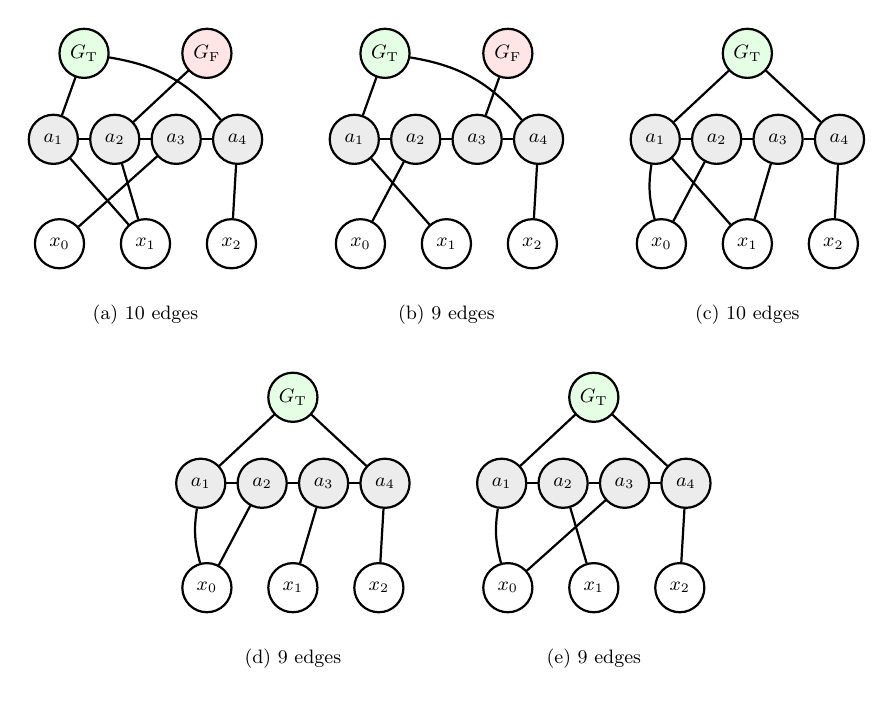
\begin{tikzpicture}[scale=0.78, transform shape,
    lit/.style={circle, draw, thick, minimum size=0.8cm, inner sep=0pt, font=\small},
    aux/.style={circle, draw, thick, fill=gray!15, minimum size=0.8cm, inner sep=0pt, font=\small},
    anct/.style={circle, draw, thick, fill=green!10, minimum size=0.8cm, inner sep=0pt, font=\small\bfseries},
    ancf/.style={circle, draw, thick, fill=red!10, minimum size=0.8cm, inner sep=0pt, font=\small\bfseries},
    edge/.style={thick},
    plab/.style={align=center, font=\small}
]
    % ---- (a) 10 edges, G_F used
    \begin{scope}[shift={(0,0)}]
        \node[anct] (GT) at (0.4,3.1) {$\GT$};
        \node[ancf] (GF) at (2.4,3.1) {$\GF$};
        \node[aux] (a1) at (-0.1,1.7) {$a_1$};
        \node[aux] (a2) at (0.9,1.7) {$a_2$};
        \node[aux] (a3) at (1.9,1.7) {$a_3$};
        \node[aux] (a4) at (2.9,1.7) {$a_4$};
        \node[lit] (x0) at (0,0) {$x_0$};
        \node[lit] (x1) at (1.4,0) {$x_1$};
        \node[lit] (x2) at (2.8,0) {$x_2$};
        \draw[edge] (a1)--(a2)--(a3)--(a4);
        \draw[edge] (a1)--(GT);
        \draw[edge] (a4) to[bend right=20] (GT);
        \draw[edge] (a2)--(GF);
        \draw[edge] (a1)--(x1); \draw[edge] (a2)--(x1);
        \draw[edge] (a3)--(x0); \draw[edge] (a4)--(x2);
        \node[plab] at (1.4,-1.15) {(a) 10 edges};
    \end{scope}
    % ---- (b) 9 edges, G_F used
    \begin{scope}[shift={(4.9,0)}]
        \node[anct] (GT) at (0.4,3.1) {$\GT$};
        \node[ancf] (GF) at (2.4,3.1) {$\GF$};
        \node[aux] (a1) at (-0.1,1.7) {$a_1$};
        \node[aux] (a2) at (0.9,1.7) {$a_2$};
        \node[aux] (a3) at (1.9,1.7) {$a_3$};
        \node[aux] (a4) at (2.9,1.7) {$a_4$};
        \node[lit] (x0) at (0,0) {$x_0$};
        \node[lit] (x1) at (1.4,0) {$x_1$};
        \node[lit] (x2) at (2.8,0) {$x_2$};
        \draw[edge] (a1)--(a2)--(a3)--(a4);
        \draw[edge] (a1)--(GT);
        \draw[edge] (a4) to[bend right=20] (GT);
        \draw[edge] (a3)--(GF);
        \draw[edge] (a1)--(x1); \draw[edge] (a2)--(x0); \draw[edge] (a4)--(x2);
        \node[plab] at (1.4,-1.15) {(b) 9 edges};
    \end{scope}
    % ---- (c) 10 edges
    \begin{scope}[shift={(9.8,0)}]
        \node[anct] (GT) at (1.4,3.1) {$\GT$};
        \node[aux] (a1) at (-0.1,1.7) {$a_1$};
        \node[aux] (a2) at (0.9,1.7) {$a_2$};
        \node[aux] (a3) at (1.9,1.7) {$a_3$};
        \node[aux] (a4) at (2.9,1.7) {$a_4$};
        \node[lit] (x0) at (0,0) {$x_0$};
        \node[lit] (x1) at (1.4,0) {$x_1$};
        \node[lit] (x2) at (2.8,0) {$x_2$};
        \draw[edge] (a1)--(a2)--(a3)--(a4);
        \draw[edge] (a1)--(GT);
        \draw[edge] (a4)--(GT);
        \draw[edge] (a1) to[bend right=12] (x0);
        \draw[edge] (a1)--(x1);
        \draw[edge] (a2)--(x0); \draw[edge] (a3)--(x1); \draw[edge] (a4)--(x2);
        \node[plab] at (1.4,-1.15) {(c) 10 edges};
    \end{scope}
    % ---- (d) 9 edges
    \begin{scope}[shift={(2.4,-5.6)}]
        \node[anct] (GT) at (1.4,3.1) {$\GT$};
        \node[aux] (a1) at (-0.1,1.7) {$a_1$};
        \node[aux] (a2) at (0.9,1.7) {$a_2$};
        \node[aux] (a3) at (1.9,1.7) {$a_3$};
        \node[aux] (a4) at (2.9,1.7) {$a_4$};
        \node[lit] (x0) at (0,0) {$x_0$};
        \node[lit] (x1) at (1.4,0) {$x_1$};
        \node[lit] (x2) at (2.8,0) {$x_2$};
        \draw[edge] (a1)--(a2)--(a3)--(a4);
        \draw[edge] (a1)--(GT);
        \draw[edge] (a4)--(GT);
        \draw[edge] (a1) to[bend right=12] (x0);
        \draw[edge] (a2)--(x0); \draw[edge] (a3)--(x1); \draw[edge] (a4)--(x2);
        \node[plab] at (1.4,-1.15) {(d) 9 edges};
    \end{scope}
    % ---- (e) 9 edges
    \begin{scope}[shift={(7.3,-5.6)}]
        \node[anct] (GT) at (1.4,3.1) {$\GT$};
        \node[aux] (a1) at (-0.1,1.7) {$a_1$};
        \node[aux] (a2) at (0.9,1.7) {$a_2$};
        \node[aux] (a3) at (1.9,1.7) {$a_3$};
        \node[aux] (a4) at (2.9,1.7) {$a_4$};
        \node[lit] (x0) at (0,0) {$x_0$};
        \node[lit] (x1) at (1.4,0) {$x_1$};
        \node[lit] (x2) at (2.8,0) {$x_2$};
        \draw[edge] (a1)--(a2)--(a3)--(a4);
        \draw[edge] (a1)--(GT);
        \draw[edge] (a4)--(GT);
        \draw[edge] (a1) to[bend right=12] (x0);
        \draw[edge] (a2)--(x1); \draw[edge] (a3)--(x0); \draw[edge] (a4)--(x2);
        \node[plab] at (1.4,-1.15) {(e) 9 edges};
    \end{scope}
\end{tikzpicture}

\medskip
\raggedright\small
Valid clause gadgets for $C=(x_0\lor x_1\lor x_2)$ with four auxiliary
vertices $a_1,\dots,a_4$, one for each of the five classes up to relabeling
the auxiliary vertices and the literals. In every class the auxiliary
vertices form a path whose two ends are adjacent to $\GT$. None of them is
$S_3$-symmetric, and no valid gadget has three or fewer auxiliary vertices.
The palette triangle, the vertex $\GB$, and its edges to the literals are
omitted; the edge counts exclude them.
\end{document}
